Subdivision algorithms contain two major
components: \emph{\tr} and \emph{\gm}.
The \tr\ reparameterizes the source mesh into the target 
mesh. The \gm\ transforms a submesh on the source mesh
to a vertex on the refined mesh. The source submesh with
the normalized weighting is called 
\emph{stencil}. A proper combination of a \tr\ and a set of 
rules of \gm\ define a valid subdivision scheme.

Figure \ref{fig:RefSchemes} shows the local configuration 
of four major refinements
employed in subdivision algorithms, which include Catmull-Clark
subdivision (PQQ) \cite{cc}, Loop subdivision (PTQ) \cite{loop},
Doo-Sabin subdivision (DQQ) \cite{ds} and $\sqrt{3}$ subdivision
\cite{sqrt3}. Subdivisions, such as Quad-Triangle subdivision (PQQ and
PTQ) \cite{qts,l-pg-03}, may employ a hybrid refinement consisting
of two different refinements.
\begin{figure}
  \centering
  \psfrag{PQQ}[]{\scriptsize PQQ} 
  \psfrag{PTQ}[]{\scriptsize PTQ}
  \psfrag{DQQ}[]{\scriptsize DQQ} 
  \psfrag{Sqrt3}[]{\scriptsize $\sqrt{3}$} 
  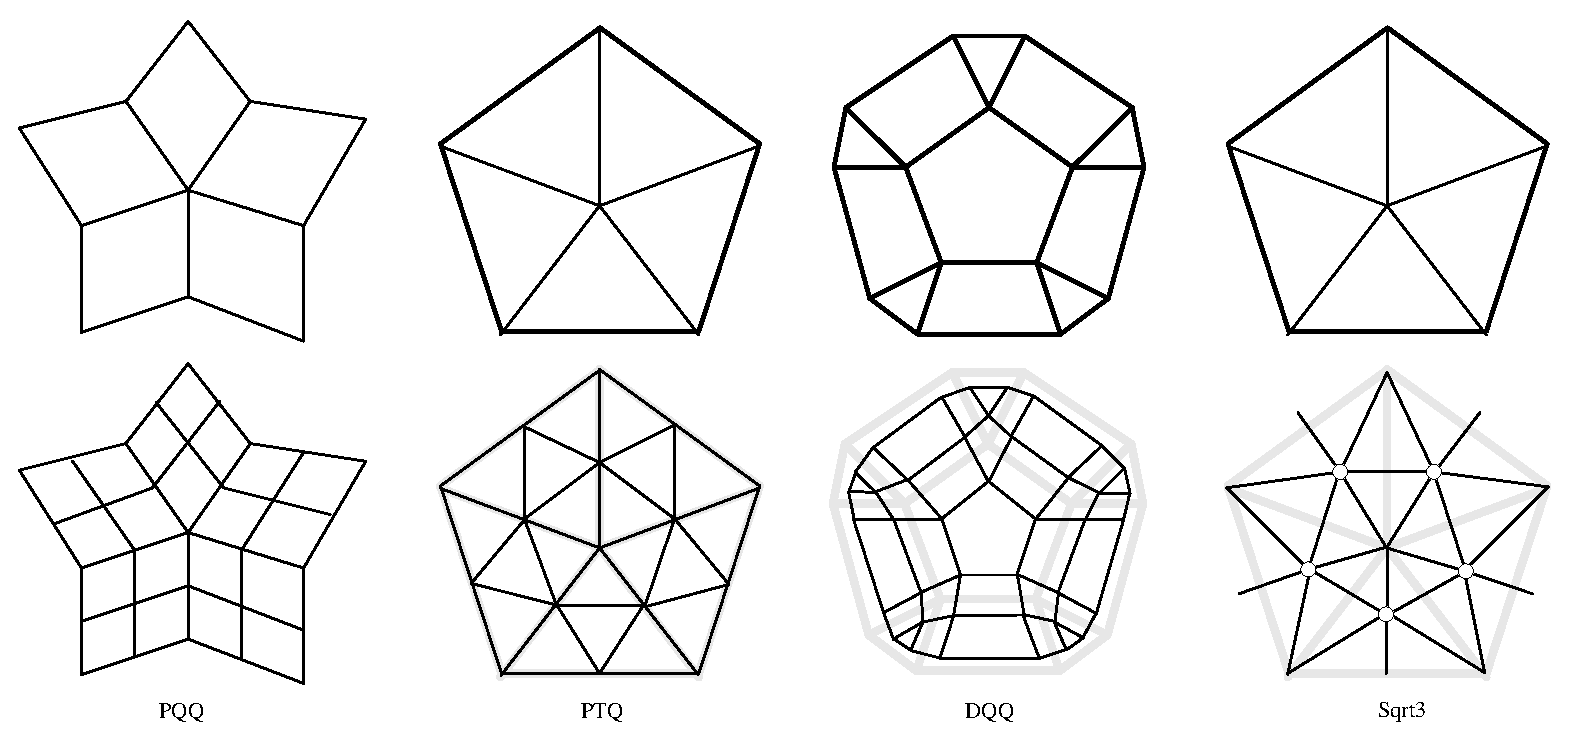
\epsfig{file=figs/RefSchemes.eps, width=7cm}
  \caption{Topology refinements: 
    primal quadrilateral quadrisection (PQQ),
    primal triangle quadrisection (PTQ),
    dual quadrilateral quadrisection (DQQ) and
    $\sqrt{3}$ triangulation.}
  \label{fig:RefSchemes}
\end{figure}
The \gm\ applies a \emph{mask} on the stencil and
generate the corresponding vertex on the refined mesh.
The mask usually specifies an affine combination of the 
stencil. Figure \ref{fig:RefMap} demonstrates the examples of the
correspondence between a stencil and its vertex. Subdivisions 
usually have distinct masks associated with different stencils 
(Figure \ref{fig:RefMap} (a-c)). 
\begin{figure}
  \centering
  \psfrag{A}[]{(a)}
  \psfrag{B}[]{(b)}
  \psfrag{C}[]{(c)}
  \psfrag{D}[]{(d)}
  \epsfig{file=figs/RefMap.eps, width=7cm}
  \caption{The stencil and its vertex in the 
           Catmull-Clark subdivision (a-c)
           and Doo-Sabin subdivision (d). Catmull-Clark
           subdivision has three stencils: facet-stencil (a), 
           edge-stencil (b) and vertex-stencil (c). 
           Doo-Sabin subdivision has only corner-stencil (d).}
  \label{fig:RefMap}
\end{figure}


% templated rules: a generic framework for subdivisions 
%\subsection{Generic Subdivisions}
%\label{sec:subtempl}
\input subtempl

\subsection{Sqrt 3}
% connectivity ops: specific polyhedron algorithms (sqrt3 subdivisions) 
%\subsection{$\sqrt{3}$-Subdivision using Euler Operators}
\input sqrt3

% inc builder: specific polyhedron algorithms (qt subdivisions) 
%\subsection{Quad-triangle Subdivision using modifier}
%\input qt

